\section{Heavy Flavor Production and Spectroscopy }

% We were thinking that it might be best if the separate sections have
% some uniformity in the way they are constructed, so as a rough
% guideline (proposed by Olivier) maybe you could ai for something like
% this:
%
%  - general introduction and motivation
%  - past and current work in the French community
%  - proposed work in the 4 coming years
%
% Note that the general introduction and motivation shouldn’t be too
% general as there will be an introductory section earlier in the
% document. Also try and be somewhat specific if possible as to the
% (recent) past and current work going on within the French community
% and why there is a need to continue and strengthen this effort.
%
% As for the length there is no length limit defined by the CNRS.
% We had mentioned a page but in words I think about 800-1000 words
% per section would be appropriate. This is of course a very rough
% guideline so you don’t need to keep to it too strictly.

%\subsection{Introduction and motivation}

Quantum Chromodynamics (and the quark model out of which it grew)
is one of the fundamental building blocks of the Standard Model.
It has been extensively validated over the decades, and is
very well understood. However, due to the non-perturbative behaviour
that follows from the large self-coupling of low-energy gluons,
the practical implications of QCD are still
very much an active subject of research. This was vividly illustrated
in the realm of spectroscopy recently, when the first compelling
observation of pentaquark ($qqqq\bar{q}$) states was made by LHCb~[\cite{Aaij:2015tga}]
just over fifty years after their existence was predicted [\cite{GellMann:1964nj}].
This discovery came as a surprise to experimentalists and theorists alike:
the possible existence of such states was known, but the quark composition of
quasi-stable pentaquark resonances (let alone their masses, widths, and
production mechanisms) was not.

More broadly, results from QCD and strong physics are frequently
needed as inputs to other measurements or to their interpretation.
For example, there is considerable interest in the decays
$\Bbar \to D^{(*)} \lepton^- \neulb$: the ratio of branching fractions
(in a restricted region of phase space) for $\lepton=\muon$ and $\lepton=\tauon$
can be used to test lepton universality. The current world average,
combining results from LHCb, BABAR and Belle, is in tension
at the $4\sigma$ level with Standard Model expectations~\cite{bib:hfag}.
One of the important systematic uncertainties in this measurement
is associated with the spectrum and properties of excited charm resonances $D^{**}$,
which could contaminate the final state with feed-down from
$\Bbar \to D^{**} \lepton^- \neulb$: here, input from spectroscopy is
needed for the measurement itself. There are numerous instances
in which QCD input is needed for the interpretation of measurements,
notably for $\Bz \to \Kstarz \mup \mun$ in which 
%local tensions of $3\sigma$ were seen by LHCb in two regions of phase space~[\cite{Aaij:2015oid}], corresponding to an overall tension of $3.4\sigma$ with the SM prediction of~\cite{Descotes-Genon:2014uoa}. 
\textcolor{red}{an overall tension of $3.4\sigma$ with the SM prediction of~\cite{Descotes-Genon:2014uoa} has been seen.}  
The significance of this 
tension depends strongly upon the SM theory prediction and its
uncertainties. To take a third and final example, QCD processes are
an inherent background to all physics at the LHC, and in some cases
Monte Carlo predictions of their spectrum need to be included in the
fit itself. Tuning of the Monte Carlo models requires not only work
from the phenomenology community but also measurements of production
cross-sections across a range of transverse momentum and
pseudorapidity.

%\subsection{(Past and current work in the French community)}

% Alphabetic ordering: CPPM > LPC > LAL > LAPP > LPNHE

The HEP community in France is engaged in this field, both on
the experimental and theory sides. For practical reasons most
experimental measurements have come from LHCb in recent years.
LHCb-France has been involved on multiple fronts:
spectroscopy of exotica,  %(LAL, LAPP, LPNHE),
spectroscopy of non-exotic resonances %(LAL, LPNHE),
and measurements of production rates.  %(CPPM, LAL, LAPP, LPNHE).
This list is not exhaustive, and there are far too many
results to discuss them individually; purely by way of
illustration we point to recent contributions by French groups to
%
studies of exotic 4- and 5-quark resonances
[\cite{Aaij:2016ymb}, \cite{Aaij:2014jqa}],
%
discoveries of two $\Xi_b$ resonances and precise measurements
of their mass splittings [\cite{Aaij:2016jnn}, \cite{Aaij:2014yka}],
%
and measurements of the $J/\psi$ production cross-section
with the new 13\,TeV LHC data
[\cite{Aaij:2015rla}].
Numerous theory groups are also actively involved, and
we do not dare attempt an exhaustive list%\footnote{  In the author list of one review paper of heavy flavour  production alone [\cite{Andronic:2015wma}],  we counted eight French laboratories:  IPNO, IRFU, LAL, LAPTh, LLR, LPC, LPSC, and SUBATECH.}.
As well as hadron production, there is substantial French
expertise in spectroscopy theory. For example, the opening
theory review talk at the 
2014 Workshop on Heavy Quark Baryons at LHCb\footnote{
  \url{https://indico.cern.ch/event/317758/}
}, a workshop organised by LHCb to which external experts were invited,
was given by a member of IPNL. This is both recognition of
this expertise and an illustration of the demand for
productive \textcolor{red}{exchanges between theory and experiments.}
%theory-experiment crosstalk.

% Note that IPNL = IPN Lyon (vs IPN at Orsay)
%
% IPNL includes Jean-Marc Richard, an expert on hadron spectroscopy

% Note especially : arXiv:1407.8526

%\subsection{(proposed work in the 4 coming years)}

During the coming years, several analyses in this area are
planned by LHCb-France and will be followed in the framework of the GDR. 
\textcolor{red}{By way of example, these include:}

\begin{itemize}
\item Studies in beauty baryon spectroscopy following on from the observations
of three $\Xi_b$ resonances;
\item Searches for the doubly heavy
$\Xi_{cc}$ baryons;
\item Measurements of production cross-sections
at new centre-of-mass energies (including the 13\,TeV Run-2
data and in heavy-ion collisions).
\end{itemize}

Assuming that the $\Xi_{cc}$
searches are successful, they in particular will lead to fruitful
exchanges with theory: their masses and properties will have
immediate implications for QCD models, and theory input will be
very useful for the next step, namely observing and studying their
excitations.




\begin{figure}[!htb]
\begin{center}
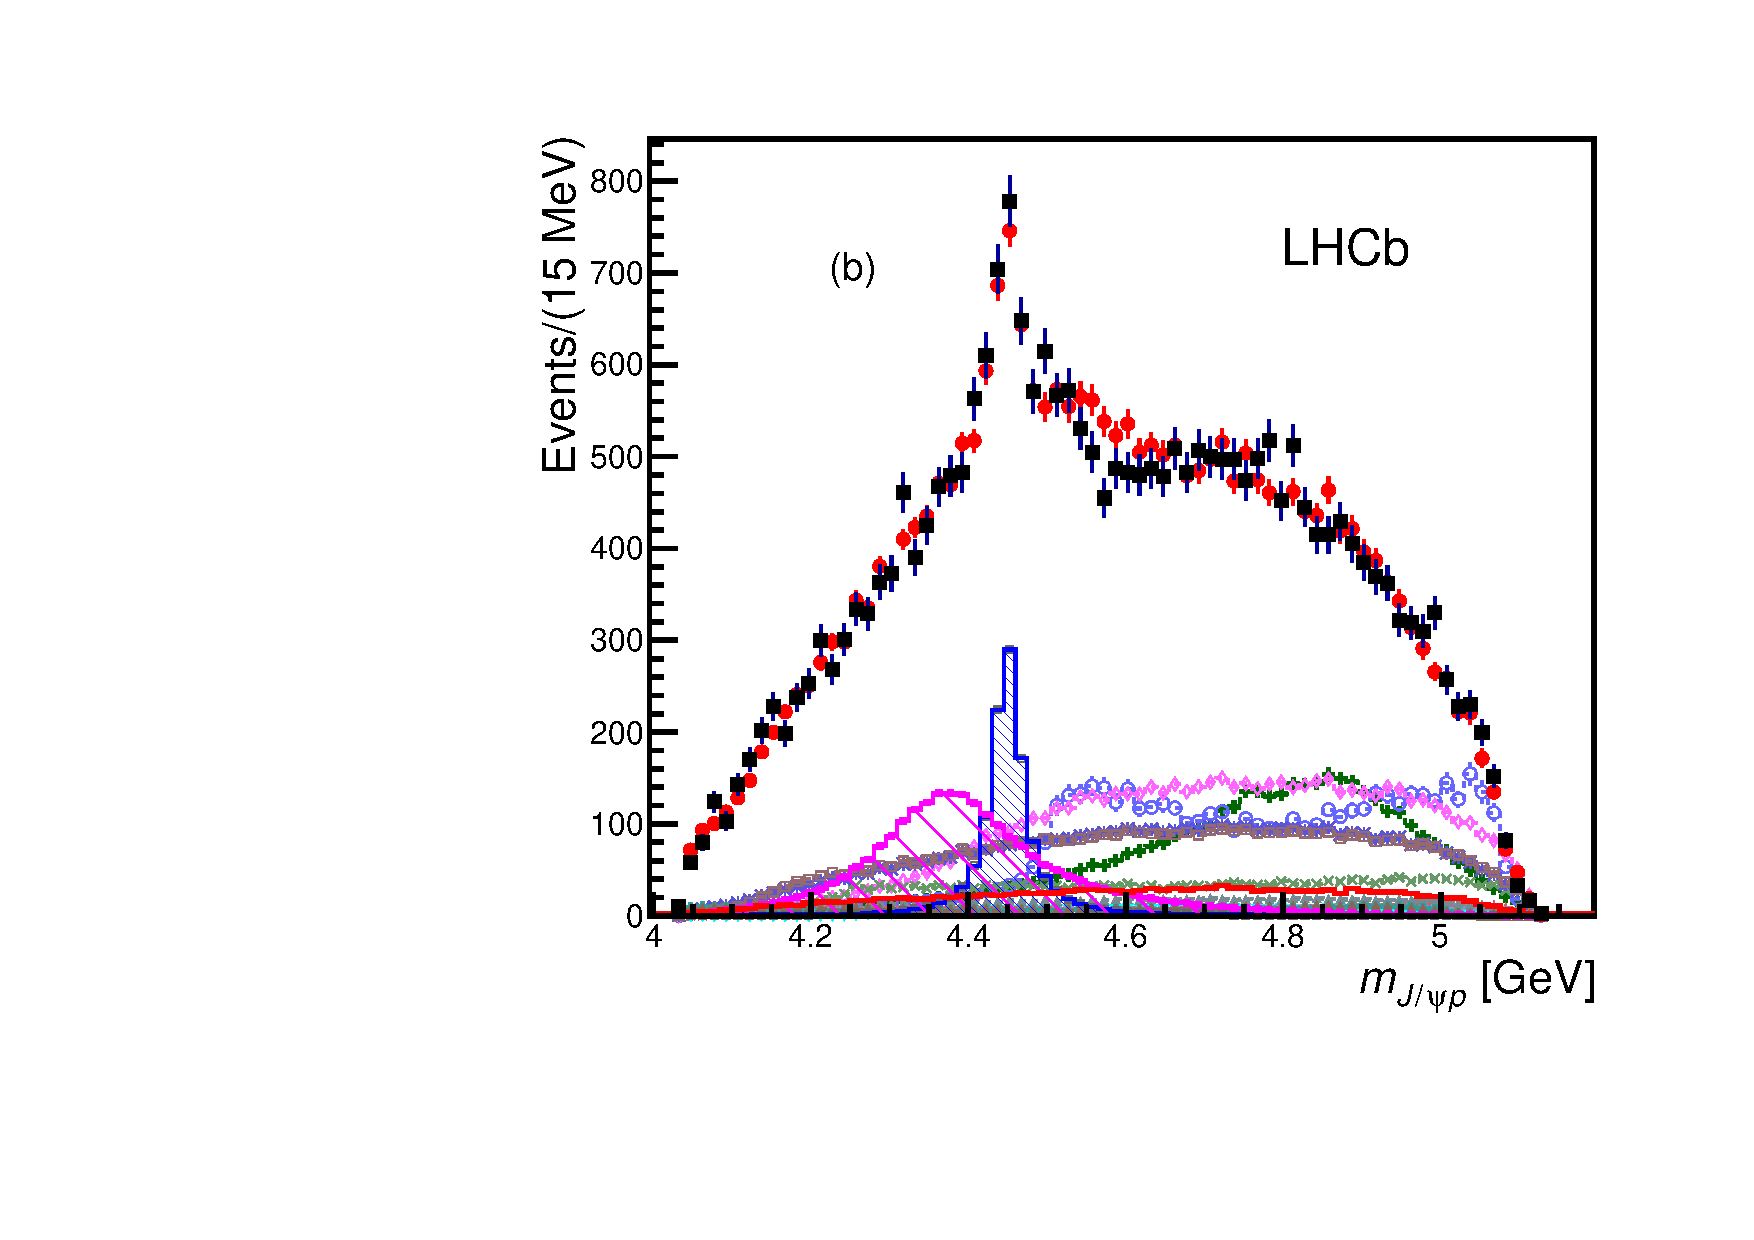
\includegraphics[width=7.5cm]{mjpsip-default.pdf} 
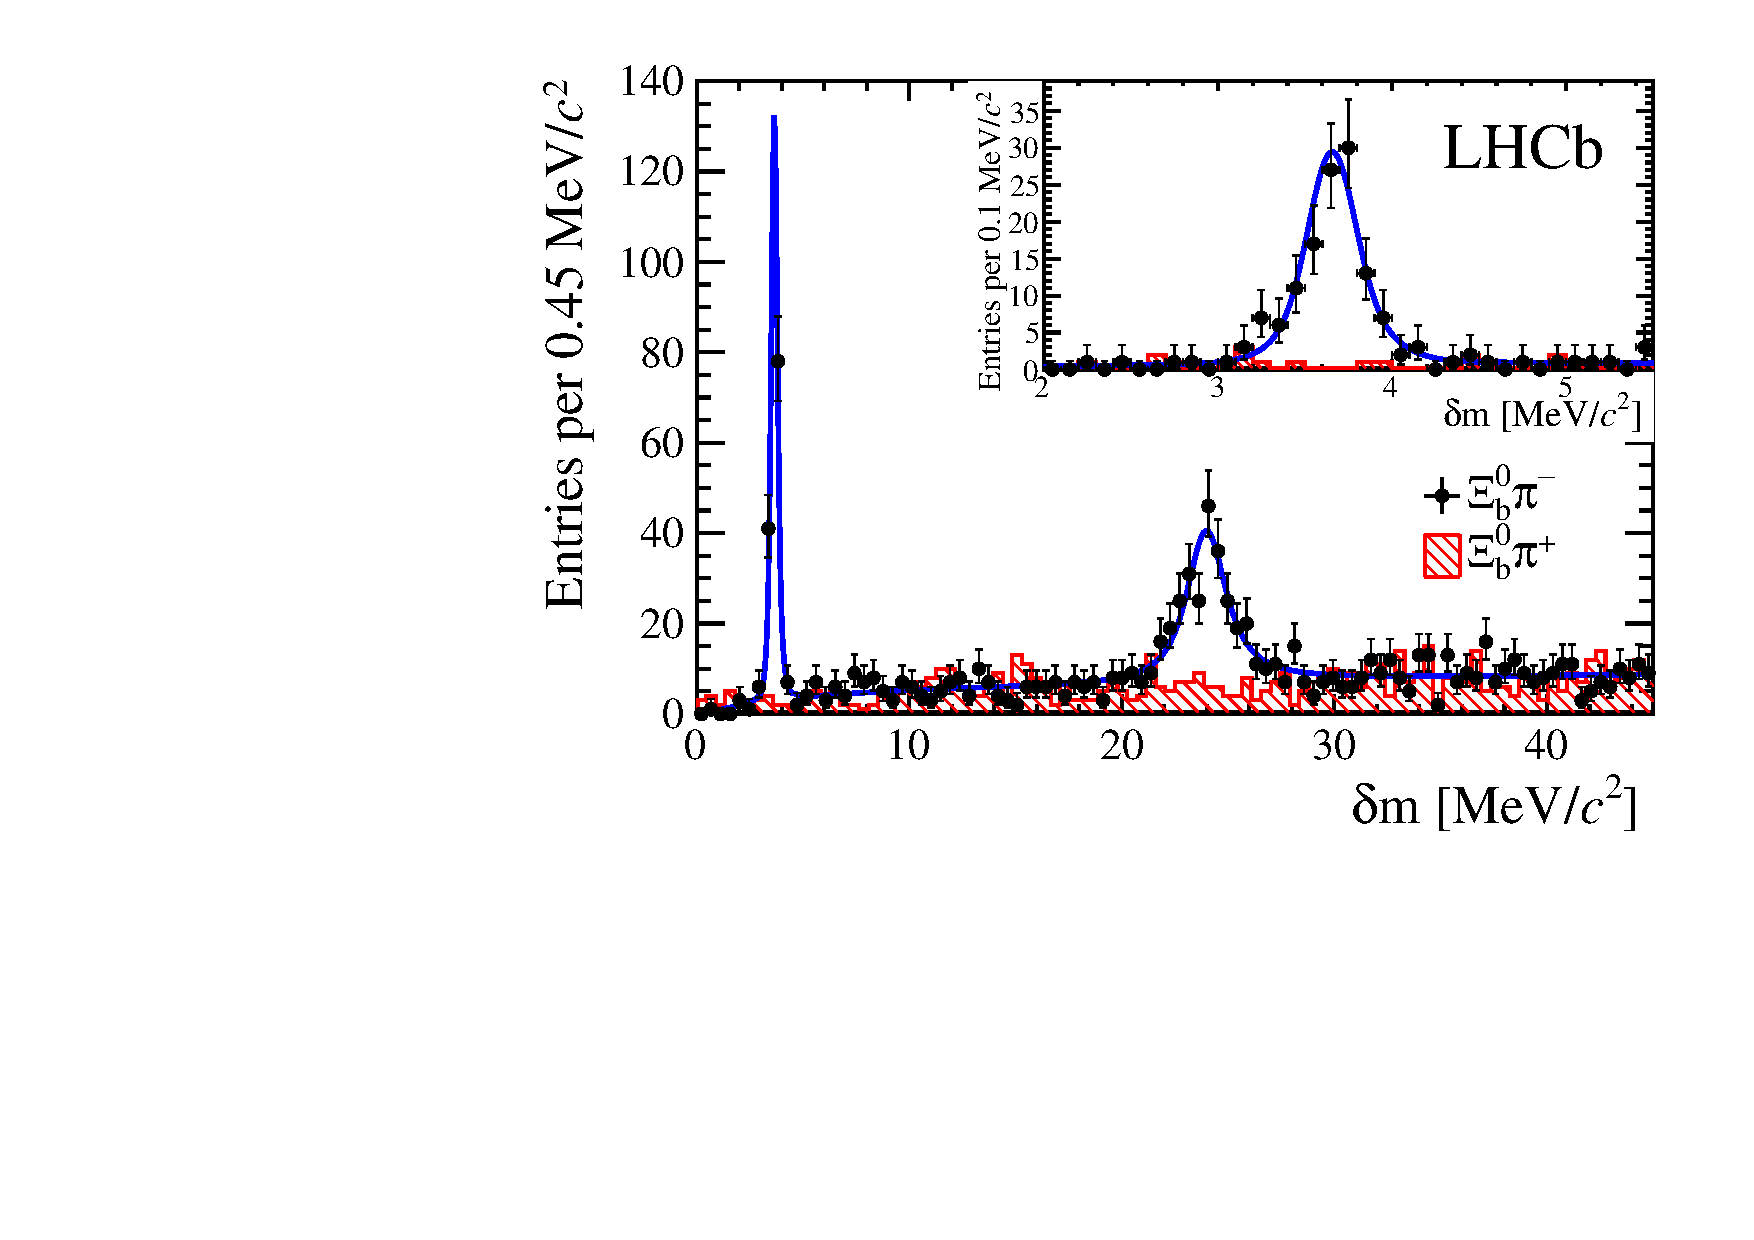
\includegraphics[width=7.5cm]{paperPlot-merged.pdf}
\end{center}
\caption{Left: Results of a fit to $\Lb \to \jpsi \Km \proton$ decays in the Run 1 LHCb data. The figure is taken from Ref.~\cite{PAPER-2015-029}, which reported the first observation of these two pentaquark states, the $P_c(4380)^+$ and $P_c(4450)^+$. Their amplitudes are shown as hatched magenta and blue histograms.  Right: Results of a fit to the $\Xibz \pim$ spectrum in the Run 1 LHCb data. The figure is taken from Ref.~\cite{PAPER-2014-061}, which reported the first observation of these two resonances, the \XibPrimeMinus and \XibStarMinus. Inset: zoom around the first peak.}%
\label{figphis}%
\end{figure}




% fin